         \chapter{Die deeltjies waaruit stowwe bestaan}\fancyfoot[LO,RE]{Chemie: Matter en materials}
\label{chap:composition}
    \setcounter{figure}{1}
    \setcounter{subfigure}{1}
    \label{m38120}
\section{Atome en verbindings}
    \subsection*{Atome is die boustene van materie}
            \nopagebreak
            \label{m38120*cid2} $ \hspace{-5pt}\begin{array}{cccccccccccc}   \end{array} $ \hspace{2 pt}\raisebox{-0.2em}{
\includegraphics[height=1em]{../icons/www.pdf}} {(section shortcode: P10053 )} \par 
      \label{m38120*id307092}Ons het gesien dat verskillende stowwe (materiale) verskillende eienskappe het. Sommige stowwe is metale ander is nie-metale, sommige stowwe is elektriese of termiese geleiers, terwyl ander nie elektrisiteit of warmte gelei nie. Afhangende van die eienskappe is daar ‘n verskeidenheid van toepassingsmoontlikhede vir hierdie stowwe. Maar waaruit bestaan hierdie stowwe regtig? Met ander woorde, wat gaan ons vind as ons ‘n stof sou afbreek in die dele waaruit dit opgebou is? En hoe is dit moontlik dat ‘n stof se mikroskopiese struktuur (die klein onsigbare dele waaruit die stof bestaan) in staat is om al die verskillende eienskappe te gee? \par 
\begin{minipage}{.6\textwidth}
      \label{m38120*id307099}
Die antwoord l\^{e} in die kleinste bousteen van materie: die \textbf{atoom}. Dit is die \textbf{soort} atome, en die manier waarop hulle is in ‘n stof \textbf{gerangskik} is wat die eienskappe van daardie stof beїnvloed. Dit stem ooreen met boumateriaal. Ons kan bakstene, staal, sement, hout, dekstrooi (vir ‘n dak), modder en baie ander materiale gebruik om strukture mee te bou. Netsoos die keuse van boumateriaal die eienskappe van die struktuur beïnvloed, beïnvloed die verskillende atome waaruit materie opgebou is die eienskappe van materie.\par 
\end{minipage}
\begin{minipage}{.4\textwidth}
 \begin{center}
\includegraphics[width=0.6\textwidth]{photos/atom_model_kit.jpg}
 \end{center}
\end{minipage}

      \label{m38120*id307459}
Stowwe kom gewoonlik nie in atoomvorm voor nie (net soos wat jy selde 'n gebou of struktuur kry wat van een soort boumateriaal gemaak is). Meeste atome is aan ander atome  gebind (geheg) om \textbf{verbindings} of \textbf{molekule} te vorm. Dit is slegs by die \textsl{edelgasse} (bv. helium, neon en argon) dat atome individueel (afsonderlik) is en nie aan ander atome verbind is nie.  Ons het na sommige van die redes hiervoor in vorige hoofstukke gekyk.\par \pagebreak
    \subsection*{Verbindings}
            \nopagebreak
            \label{m38120*cid3} $ \hspace{-5pt}\begin{array}{cccccccccccc}   \end{array} $ \hspace{2 pt}\raisebox{-0.2em}{
\includegraphics[height=1em]{../icons/www.pdf}} {(section shortcode: P10054 )} \par 
\par
            \label{m38120*fhsst!!!underscore!!!id74}
\Definition{ Verbinding} {'n Verbinding is' n groep van twee of meer verskillende atome wat deur relatief sterk kragte of bindings bymekaar gehou word. Die atome verbind in ‘n definitiewe verhouding.} 
Byna alles rondom ons is van verbindings gemaak. Verbindings vorm wanneer twee of meer atome in ‘n vaste verhouding aanmekaaar gebind is. Verbindings word verdeel in \textbf{molekul\^{e}re verbindings} (molekule), \textbf{ioniese verbindings} (soute) en \textbf{metaalverbindings} (metale).
\begin{itemize}[noitemsep]
 \item \textbf{Molekul\^{e}re verbindings} vorm wanneer nie-metaal-atome elektrone deel, die binding word 'n kovalente binding genoem. 
\item \textbf{Ioniese verbindings} vorm wanneer elektrone vana f metaalatome na nie-metale-atome oorgedra word, die binding word ‘n ioniese binding genoem. 
\item \textbf{Metale} word gevorm as gevolg van metaalbinding. Metaalatome verloor hulle buitenste elektrone om ‘n rooster of tralie van reëlmatig gespasieerde positiewe ione te vorm met 'n "see of poel" van gedelokaliseerde (los gemaakte) elektrone rondom die positiewe ione. 
\end{itemize}
Die volgende diagram illustreer hoe verbindings onderverdeel word in die tipe binding en die struktuur.
\begin{figure}[H]
 \begin{center}
  \begin{pspicture}(-6,0.5)(6,5)
%\psgrid[gridcolor=lightgray]
\rput(0,4.8){\textbf{VERBINDINGS}}
\psline(-3,4)(-3,4.4)(4.5,4.4)(4.5,4)
\rput(-3,3.8){\textbf{Kovalente molekul\^{e}re strukture }}
\rput(4.8,3.8){\textbf{Netwerkstrukture}}
\psline(4.5,3)(4.5,3.6)
\psline(7.5,3)(7.5,3.4)(1.5,3.4)(1.5,3)
%covalent molecular
\rput(-3,3.3){water ($\text{H}_{2}\text{O}$)}
\rput(-3,2.8){suurstof ($\text{O}_{2}$)}
\rput(-3,2.3){swawel ($\text{S}_{8}$)}
\rput(-3,1.8){buckyballe ($\text{C}_{60}$)}
%putting other text
\rput(4.5,2.8){\textbf{Ioniese-netwerk}}
\rput(4.5,2.4){\textbf{strukture}}
\rput(1.2,2.8){\textbf{Kovalente-netwerk}}
\rput(1.2,2.4){\textbf{strukture}}
\rput(7.8,2.8){\textbf{Metaalnetwerk}}
\rput(7.8,2.4){\textbf{strukture}}
%ionic structures
\rput(4.5,1.9){natriumchloried ($\text{NaCl}$)}
\rput(4.5,1.4){bariumsulfaat ($\text{BaSO}_{4}$)}
\rput(4.5,0.9){silwer jodied ($\text{AgI}$)}
%metallic structures
\rput(7.8,1.9){koper ($\text{Cu}$)}
\rput(7.8,1.4){yster ($\text{Fe}$)}
\rput(7.8,0.9){goud ($\text{Au}$)}
%other covalent
\rput(1.2,1.9){diamond ($\text{C}$)}
\rput(1.2,1.4){grafiet ($\text{C}$)}
\rput(1.2,0.9){silikondioksied ($\text{SiO}_{2}$)}
\end{pspicture}
 \end{center}
\end{figure}
\subsubsection*{Kovalente molekul\^{e}re strukture}
Relatief klein molekule word kovalente molekulêre strukture genoem en bestaan uit die wisselwerking van afsonderlike molekules op. Suurstof ($\text{O}_{2}$), water ($\text{H}_{2}\text{O}$), oktaan ($\text{C}_{8}\text{H}_{18}$), swawel ($\text{S}_{8}$) en buckminsterfullerene ($\text{C}_{60}$, buckyballe) is almal voorbeelde van kovalente molekulêre strukture. (Buckyballe - buckminsterfullerene is ‘n allotroop van koolstof vernoem na Richard Buck).\\
\begin{figure}[H]
  \begin{center}
  \begin{minipage}[c]{5 cm}
    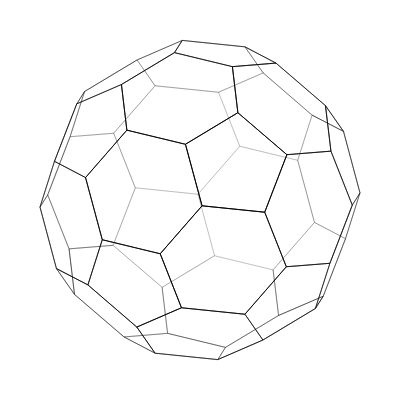
\includegraphics[width=0.6\textwidth]{photos/Buckyball_Carbon.png} \\
    \textsl{buckminsterfullerene}
  \end{minipage}
  \begin{minipage}[c]{5 cm}
    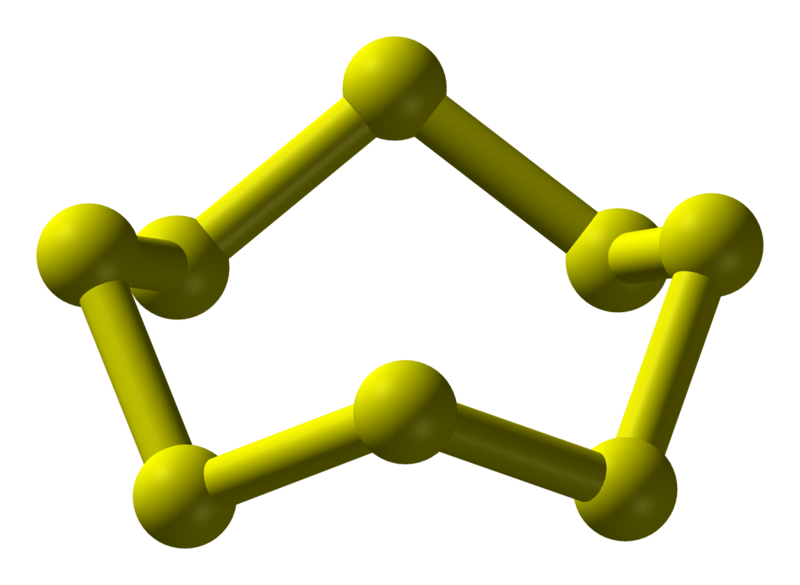
\includegraphics[width=0.6\textwidth]{photos/sulphur_wikipedia.png}  \\ 
    \textsl{swawel}
  \end{minipage}
\caption{Voorbeelde van kovalente molekul\^{e}re strukture}
\end{center}
\end{figure}

\subsubsection*{Netwerkstrukture}
Verbindings wat slegs as reuse herhalende roosterstrukture bestaan, word netwerkstrukture genoem. Voorbeelde sluit in \textbf{kovalente molekule} soos diamant, grafiet en silikondioksied (silika). \textbf{Ioniese stowwe} is ook netwerkstrukture. 'n Natriumchloriedkristal is byvoorbeeld ‘n reuse rooster (traliewerk) van herhalende eenhede bestaande uit natrium- en chloriedione. Alle stowwe wat gevorm word as 'n gevolg van ioniese binding is netwerkstrukture. \textbf{Metale} bestaan as groot deurlopende roosterstrukture, en word dus ook as netwerkstrukture geklassifiseer. Koper, sink en yster kan byvoorbeeld gesien word as reusekristalle en word daarom beskou as netwerkstrukture.
\begin{figure}[H]
  \begin{center}
  \begin{minipage}[c]{5 cm}
    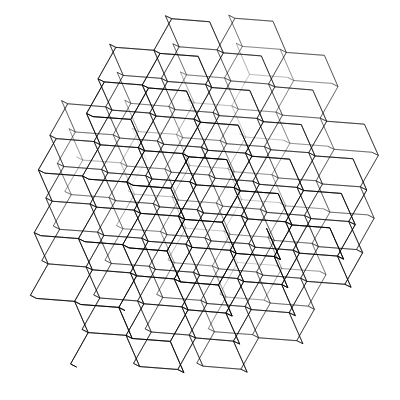
\includegraphics[width=0.8\textwidth]{photos/Diamond_Carbon.png} \\
    \textsl{Kovalente-netwerk}
  \end{minipage}
  \begin{minipage}[c]{5 cm}
    \includegraphics[width=0.8\textwidth]{photos/BaSO4_wikipedia.png}  \\ 
    \textsl{Ioniese- netwerk}
  \end{minipage}
  \begin{minipage}[c]{5 cm}
    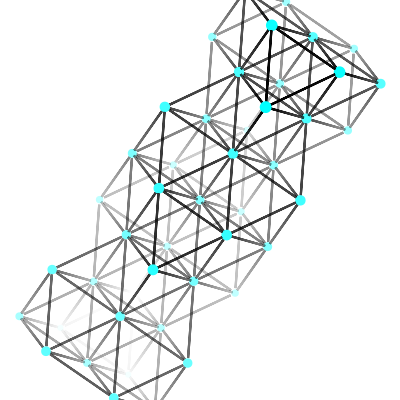
\includegraphics[width=0.8\textwidth]{photos/copper_structure.png}   \\ 
    \textsl{metaalnetwerk}
  \end{minipage}
\caption{Voorbeelde van netwerkstrukture}
\end{center}
\end{figure}
            \subsection*{Molekuulvoorstelling}
            \nopagebreak
        \label{m38120*id307557}
Die struktuur van 'n molekule kan op talle verskillende maniere getoon word. Somstyds is dit die maklikste om te wys hoe 'n molekuul lyk deur verskillende tipes \textbf{diagramme} te gebruik, maar andersins kan ons eenvoudig besluit om om 'n molekule met die \textbf{chemiese formule} of skriftelike naam voor te stel.\par 
\subsubsection*{Gebruik formules om die struktuur van 'n molekuul aan te toon.}
'n \textbf{Chemiese formule} is' n verkorte (kort) manier om 'n molekuul, of 'n ander chemiese stof, te beskryf. In die hoofstuk oor die klassifikasie van materie, het ons gesien dat chemiese verbindings voorgestel kan word deur van element se simbole op die periodieke tabel gebruik te maak. 'n Chemiese formule dui ook die \textsl{aantal} atome van elke element in 'n molekuul asook hul \textsl{verhouding} in daardie molekuul aan. Die chemiese formule vir 'n koolstofdioksied molekuul is byvoorbeeld ${\text{CO}}_{2}$. Die genoemde formule word die \textbf{molekul\^{e}re formule} van die verbinding genoem. Die formule vertel ons dat daar in een molekuul koolstofdioksied een koolstofatoom en twee suurstofatome is. Die verhouding koolstofatome tot suurstofatome is 1: 2.
\vspace{\rubberspace}\par
        \label{m38120*fhsst!!!underscore!!!id87}
 \Definition{Molekul\^{e}re formule} {This is a concise way of expressing information about the atoms that make up a particular chemical compound. The molecular formula gives the exact number of each type of atom in the molecule. } 

'n Glukose molekuul het die molekulêre formule: ${\text{C}}_{6}{\text{H}}_{12}{\text{O}}_{6}$. In elke glukose molekuul, is daar ses koolstofatome, twaalf waterstof atome en ses suurstof atome. Die verhouding van koolstof: waterstof:suurstof is 6:12:6. Ons kan hierdie verhouding vereenvoudig en skryf as 1:2:1. Dit beteken dat daar vir elke koolstofatoom twee waterstofatome en een suurstofatoom is. As ons nou die simbole van elke element  gebruik, word die formule geskryf as: ${\text{CH}}_{2}\text{O}$. Dit word die \textbf{empiriese formule} van die molekuul genoem.
\vspace{\rubberspace}\par
        \label{m38120*fhsst!!!underscore!!!id93}
\Definition{Empiriese formule} { Dit is 'n manier om die \textsl{relatiewe} getal van elke soort atoom in' n chemiese verbinding uit druk. In die meeste gevalle wys die empiriese formule nie die presiese aantal atome nie, maar eerder die eenvoudigste verhouding van die atome in die verbinding.} 

Die empiriese formule is nuttig wanneer ons die formule vir \textsl{netwerkstrukture} wil skryf. Aangesien netwerkstrukture bestaan uit miljoene atome, is dit onmoontlik om presies te sê hoeveel atome daar in elke eenheid is. Dit maak sin om dan hierdie eenhede voor te stel met behulp van hul empiriese formule. Dus in die geval van 'n metaal soos koper, skryf ons eenvoudig $\text{Cu}$, of as ons 'n molekuul natriumchloried voorstel, skryf ons net $\text{NaCl}$. Chemiese formules vertel ons iets oor die aard van die atome wat in 'n verbinding is en die verhouding waarin hierdie atome in die verbinding voorkom, maar dit gee nie vir ons enige idee van hoe die molekule eintlik lyk nie, met ander woorde sy vorm of fatsoen. Om die vorm van verbindings te illustreer kan ons diagramme gebruik. Nog 'n tipe formule wat gebruik kan word om' n verbinding te beskryf is die \textbf{struktuurformule}. 'n Struktuurformule maak gebruik van' n grafiese voorstelling om ‘n verbinding se struktuur te toon. 
(Figuur \ref{fig:representing isobutane}).
    \setcounter{subfigure}{0}
\begin{figure}[h]
\begin{center}
\begin{pspicture}(-5,-1)(5,0.6)
%\psgrid[gridcolor=lightgray]
\rput(-3,0){(a) \textbf{C$_{4}$H$_{10}$}}
\rput(-1,0){(b) \textbf{C$_{2}$H$_{5}$}}
\rput(0.5,0){(c)}
\rput(2,0){\chemfig{CH(-[2]CH_3)(-[7]CH_3)(-[5]CH_3)}}
\end{pspicture}
\caption{Diagram toon (a) die molekul\^{e}re, (b) die empiriese en (c) die struktuurformule van 2-metielpropane}
\label{fig:representing isobutane}
\end{center}
\end{figure}      
\label{m38120*uid4}\subsubsection*{Diagramme om die struktuur van 'n verbinding te toon}
Diagramme van verbindings is baie nuttig omdat hulle ons help om ‘n beeld te vorm om hoe atome in ‘n verbinding gerangskik is. Dit help ons om die vorm van die verbinding te ‘sien’. Daar is drie tipes diagramme wat algemeen gebruik word:
\label{m38120*id307860}\begin{itemize}[noitemsep]
\item \textbf{Draadraam- of stokmodelle} \\
In hierdie model, word die bindings tussen atome as 'stokkies' getoon. Hierdie "stokkies" is gekleurd om te wys watter atome verbind.
\label{m38120*uid5}\item \textbf{Bal-en stokmodelle} \\
Dit is 'n 3-dimensionele molekulêre model wat "balle" gebruik om atome voor te stel, die “stokke" stel die bindings tussen hulle voor. Die middelpunte  van die atome (die balle) is met reguit lyne verbind, dit stel die bindings voor. 
\item \textbf{Ruimtelike modelle} \\
Dit is ook 3-dimensionele molekul\^{e}re modelle. Die atome word as sfere voorgestel.
\end{itemize}
Tabel~\ref{tab:atommodels} toon voorbeelde van verskillende modelstrukture vir al die tipes verbindings.
\begin{table}[H]
 \begin{center}
  \begin{tabular}{|p{2cm}|l|l|l|l|}  \hline
   & \textbf{Kovalente molekul\^{e}re} & \textbf{Kovalente netwerk} & \textbf{Ioniese netwerk} & \textbf{Metaalnetwerk}   \\ \hline
\textbf{Naam van saamgestelde} & glukose & grafiet & silwerchloride & sink \\ \hline
\textbf{Formule} & $\text{C}_{6}\text{H}_{12}\text{O}_6$ or $\text{C}\text{H}_{2}\text{O}$ & $\text{C}$ & $\text{AgCl}$ & $\text{Zn}$  \\ \hline
\textbf{Stokmodel} & 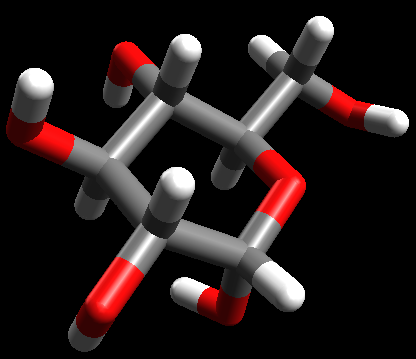
\includegraphics[width=.2\textwidth]{photos/glucose_wire.png} & \includegraphics[width=.2\textwidth]{photos/graphite.png} & \scalebox{0.5} % Change this value to rescale the drawing.
{
\begin{pspicture}(0,-1.78)(2.02,1.78)
  \psset{Alpha=75,Beta=20}
  \psset{xMin=-3,xMax=3,yMin=-3,yMax=3,zMin=-3,zMax=3}
%   \pstThreeDCoor
   \pstThreeDLine(-2,-2,-2)(-2,-2,2) \pstThreeDLine(-2,-2,2)(-2,2,2)
   \pstThreeDLine(-2,2,2)(-2,2,-2) \pstThreeDLine(-2,2,-2)(-2,-2,-2)
   \pstThreeDLine(-2,-2,0)(-2,2,0) \pstThreeDLine(-2,0,-2)(-2,0,2)

   \pstThreeDLine(0,-2,-2)(0,-2,2) \pstThreeDLine(0,-2,2)(0,2,2)
   \pstThreeDLine(0,2,2)(0,2,-2) \pstThreeDLine(0,2,-2)(0,-2,-2)
   \pstThreeDLine(0,-2,0)(0,2,0) \pstThreeDLine(0,0,-2)(0,0,2)

  \pstThreeDLine(2,-2,-2)(2,-2,2) \pstThreeDLine(2,-2,2)(2,2,2)
  \pstThreeDLine(2,2,2)(2,2,-2) \pstThreeDLine(2,2,-2)(2,-2,-2)
  \pstThreeDLine(2,-2,0)(2,2,0) \pstThreeDLine(2,0,-2)(2,0,2)

  \pstThreeDLine(-2,2,2)(2,2,2) \pstThreeDLine(-2,0,2)(2,0,2)
  \pstThreeDLine(-2,-2,2)(2,-2,2)
  \pstThreeDLine(-2,2,0)(2,2,0) \pstThreeDLine(-2,0,0)(2,0,0)
  \pstThreeDLine(-2,-2,0)(2,-2,0)
  \pstThreeDLine(-2,2,-2)(2,2,-2) \pstThreeDLine(-2,0,-2)(2,0,-2)
  \pstThreeDLine(-2,-2,-2)(2,-2,-2)
\end{pspicture} 
}  & \includegraphics[width=.15\textwidth]{photos/zinc_sticks.png} \\ \hline
\textbf{Bal-en-stokmodel} & \includegraphics[width=.2\textwidth]{photos/glucose_balls.png}  & 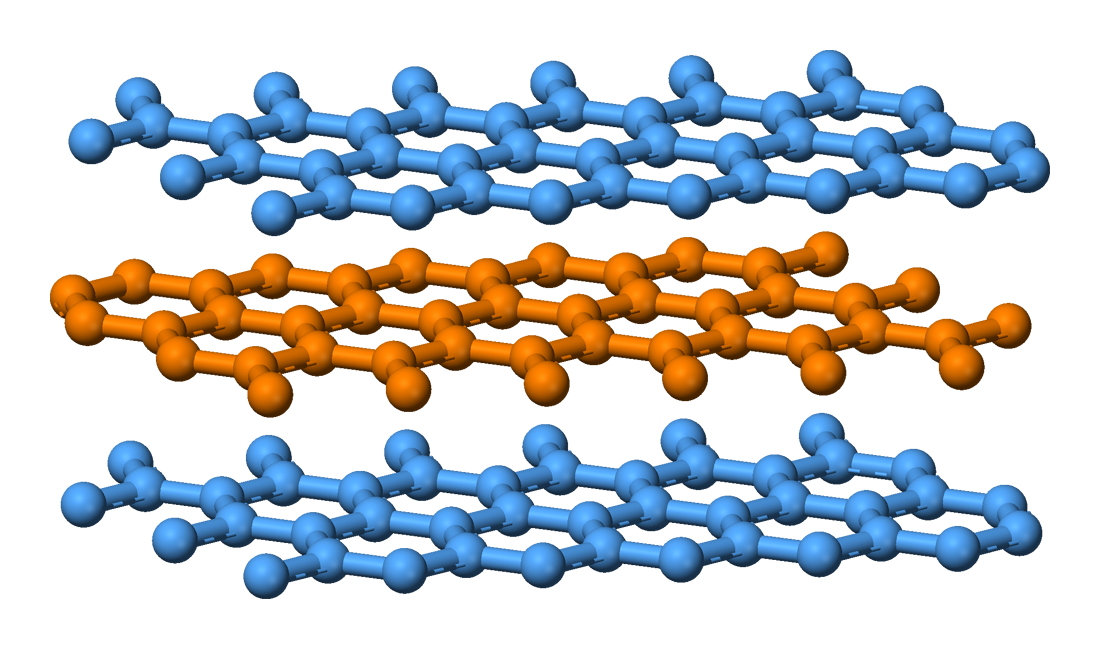
\includegraphics[width=.2\textwidth]{photos/graphite_wikipedia.png} & 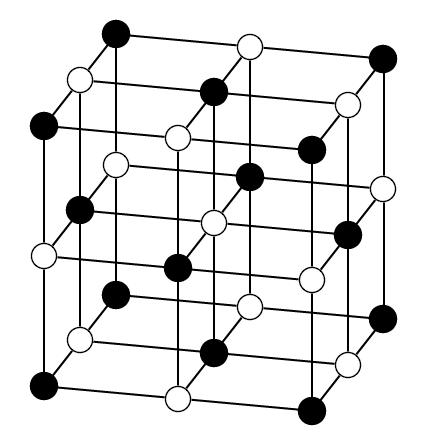
\includegraphics[width=.2\textwidth]{photos/silver_chloride_ballstick.png} & \includegraphics[width=.1\textwidth]{photos/zinc_ball_stick.png} \\ \hline
\textbf{Ruimtelike model} & \includegraphics[width=.1\textwidth]{photos/glucose_spacefill.png}  & 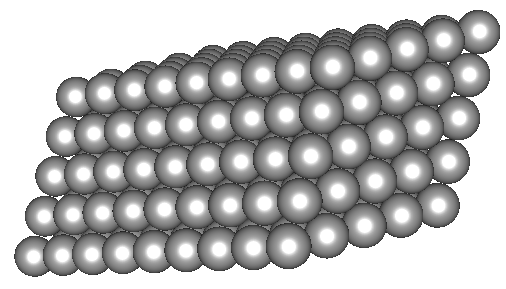
\includegraphics[width=.2\textwidth]{photos/graphite_spacefill.png} & \includegraphics[width=.1\textwidth]{photos/silverchloride_spacefill_wikipedia.png} & 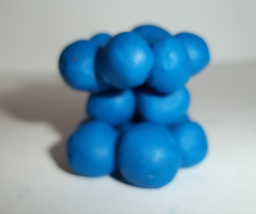
\includegraphics[width=.1\textwidth]{photos/zinc_spacefill.png} \\ \hline
  \end{tabular}
 \end{center}
\caption{Verskillende voorstellings vir verbindings}
\label{tab:atommodels}
\end{table}

\begin{activity}{Voorstelling van verbindings}
'n Lys van stowwe word hieronder gegee. Maak gebruik van die atoommodelstel, speelklei en tandestokkies, of gekleurde polistireenballe en sosatie stokkies om elk van die stowwe as drie dimensionele strukture voor te stel.\\
\begin{minipage}{.4\textwidth}
\begin{itemize}
 \item glukose ($\text{C}_{6}\text{H}_{12}\text{O}_{6}$)
\item silikondioksied ($\text{SiO}_{2}$)
\item natriumchloried ($\text{NaCl}$)
\item swawel ($\text{S}_{8}$)
\item diamant ($\text{C}$)
\item grafiet ($\text{C}$)
\item buckyballe( $\text{C}_{60}$)
\item sukrose of rietsuiker ($\text{C}_{12}\text{H}_{22}\text{O}_{11}$)
\item koper ($\text{Cu}$)
\end{itemize}
\end{minipage}
\begin{minipage}{.6\textwidth}
\begin{center}
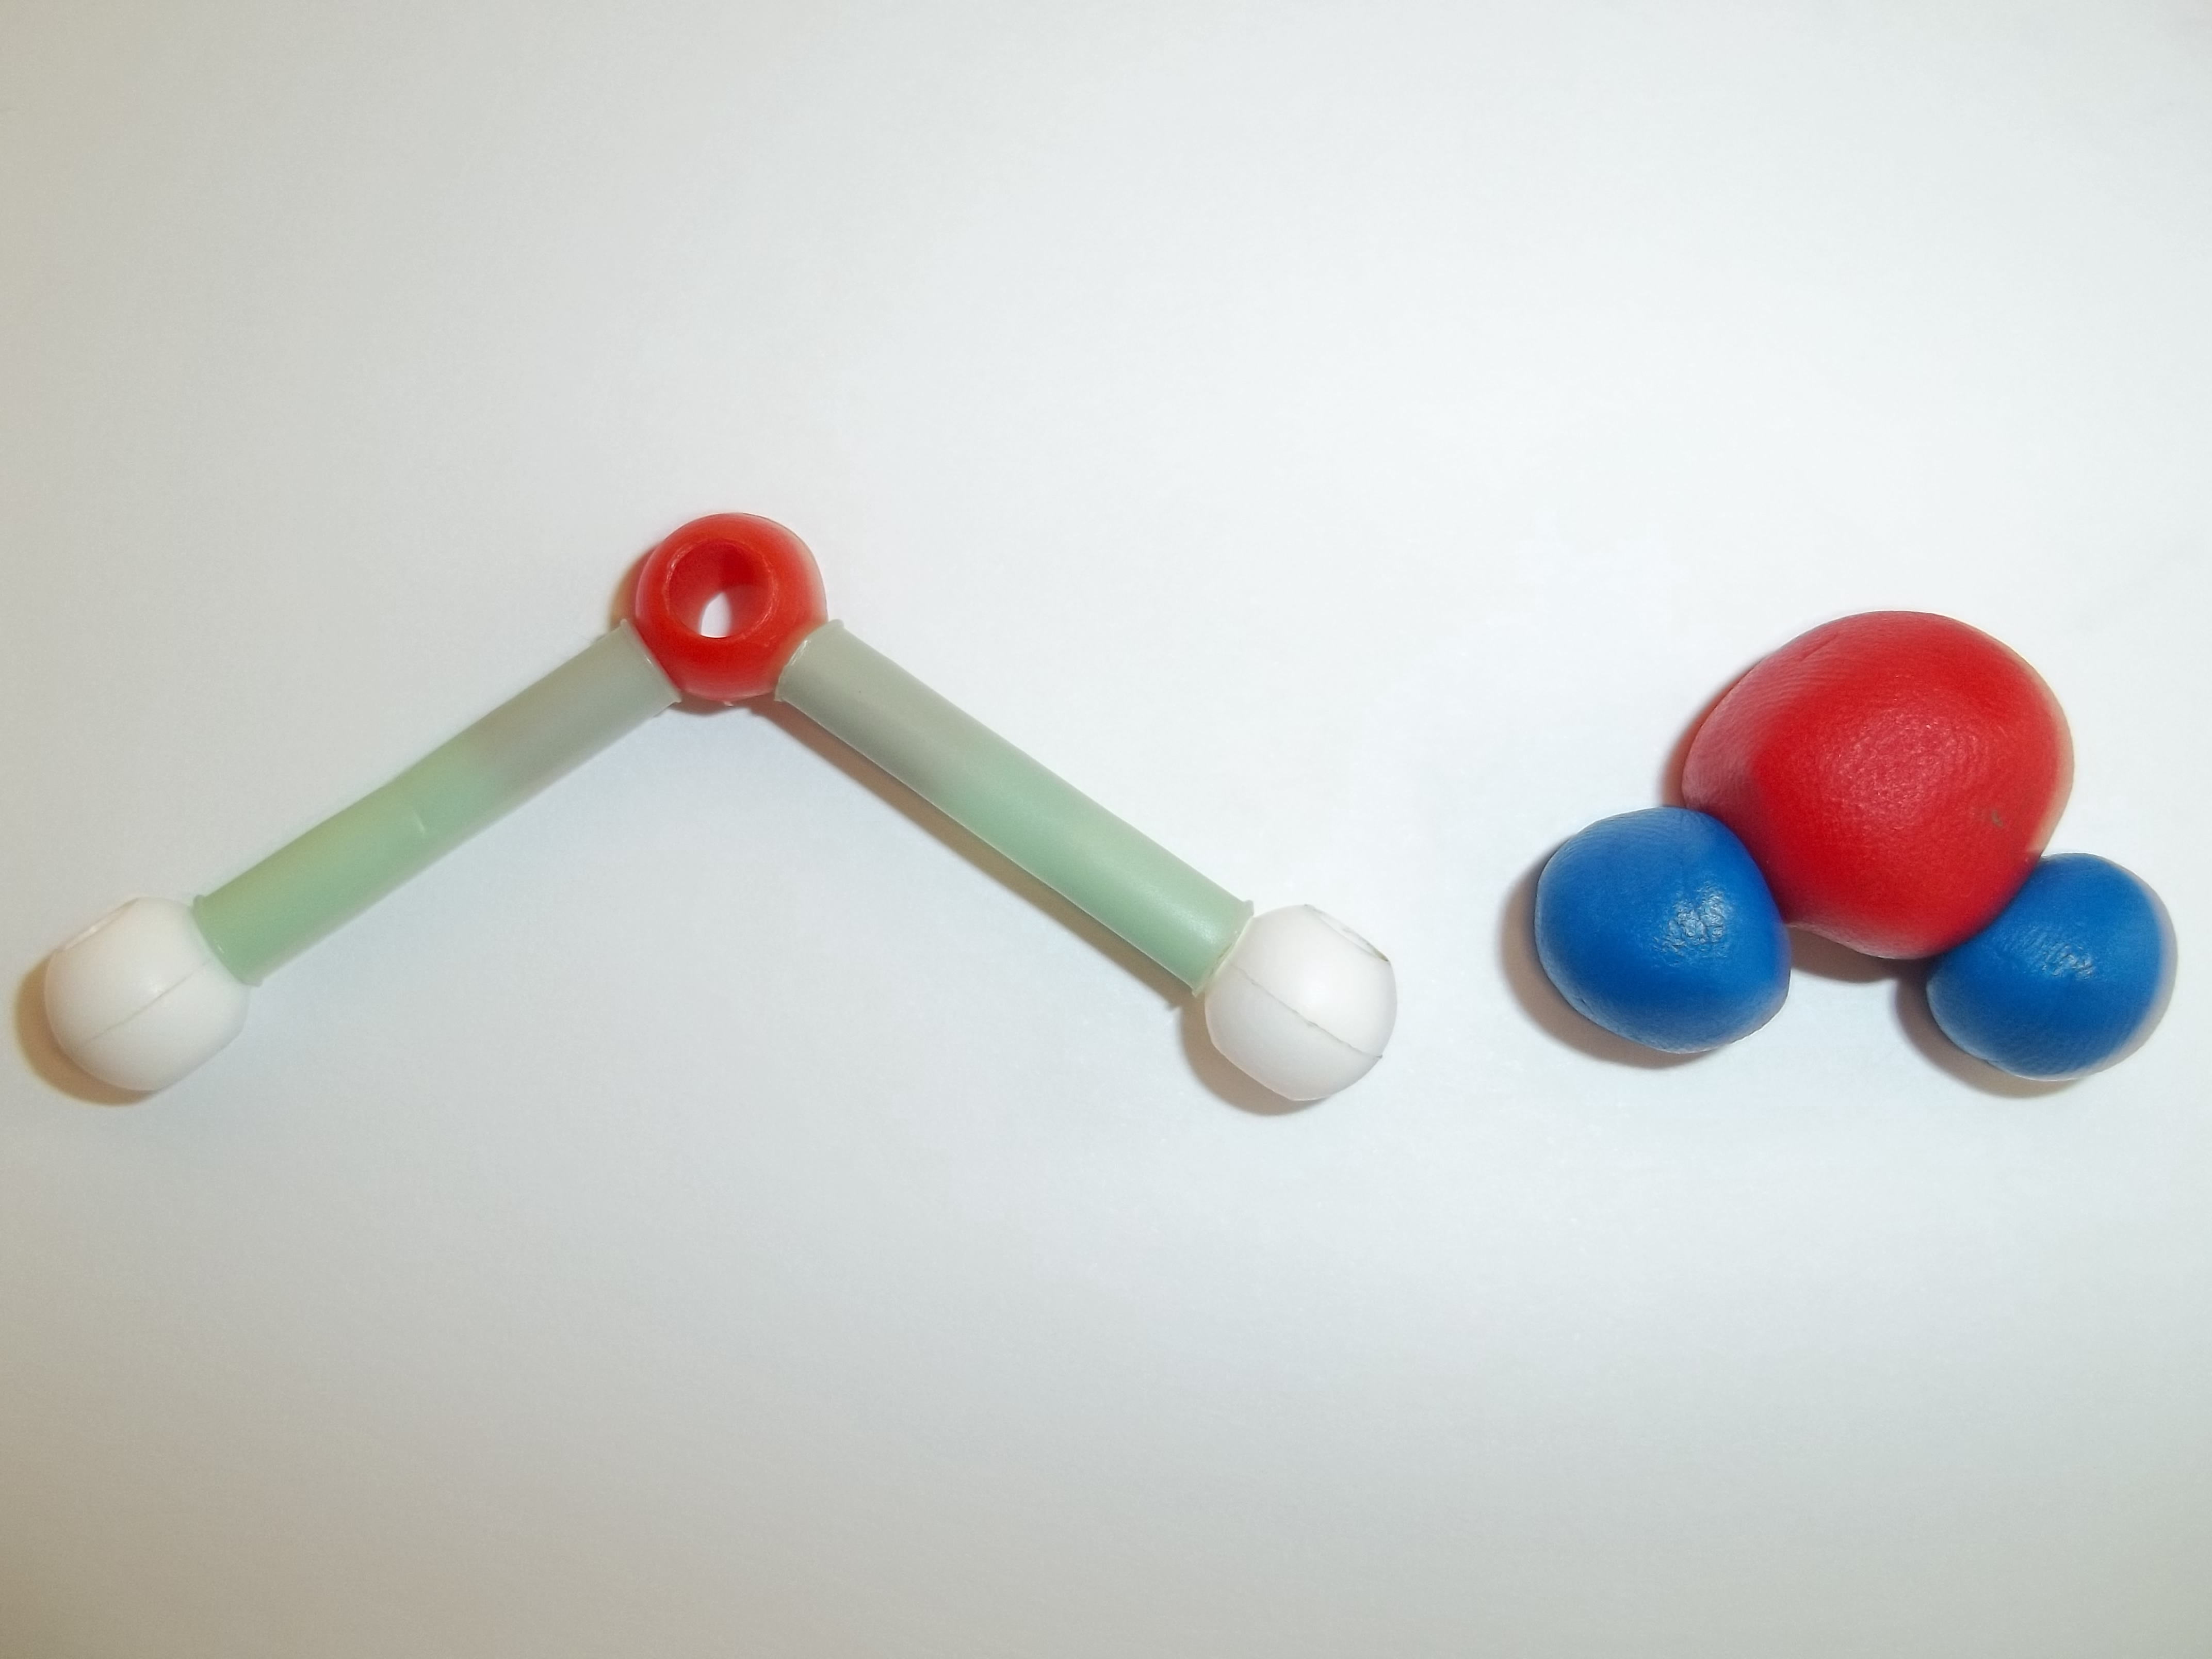
\includegraphics[width=0.4\textwidth]{photos/water.jpg}
\end{center}  
\begin{center}
\includegraphics[width=0.4\textwidth]{photos/ammonia.jpg}
\end{center}
\end{minipage}
\end{activity}
\label{m38120*uid8310432}Besoek die webwerf (http://alteredqualia.com/canvasmol/) om 'n paar verbindings te besigtig. Jy
hoef nie hierdie molekules te ken ie, dit is bloot om te sien hoe molekules voorgestel word. 
\begin{g_experiment}{Ondersoek elemente en verbindings}
 \textbf{Doel:} \\
Om te leer oor elemente en verbindings deur drie reaksies te ondersoek. \\
\textbf{Apparatus:} \\
\begin{minipage}{.5\textwidth}
\begin{itemize}[noitemsep]
 \item Cal-C-Vita tablet
\item proefbuise
\item Bunsenbrander
\item rubberprop
\item afleibuis
\item kalkwater ('n versadigde oplossing $\text{Ca(OH)}_{2}$)
\item kers
\item vuurhoutjies
\item kopersulfaat ($\text{CuSO}_{4}\cdot 10\textsf{H}_{2}\textsf{O}$)
\item sinkmetaal
\item soutsuur ($\text{HCl}$)
\end{itemize}
\end{minipage}
\begin{minipage}{.5\textwidth}
\begin{center}
\scalebox{0.9} % Change this value to rescale the drawing.
{
\begin{pspicture}(0,-1.387)(2.556,1.402)
\pspolygon[linewidth=0.03,fillstyle=solid,fillcolor=black](0.04,0.34699997)(0.62,0.34699997)(0.62,0.807)(0.04,0.807)
\rput{180.0}(0.68,-2.106){\psarc[linewidth=0.04](0.34,-1.053){0.31400025}{0.0}{180.0}}
\psline[linewidth=0.04cm](0.02,-1.0730001)(0.02,0.627)
\psline[linewidth=0.04cm](0.656,-1.0730001)(0.656,0.627)
\rput{30.256437}(-0.5475818,-0.38053852){\psellipse[linewidth=0.04,dimen=outer,fillstyle=solid,fillcolor=black](0.43,-1.2030001)(0.21,0.07)}
\psline[linewidth=0.04cm](0.0,-0.953)(0.64,-0.953)
\pscircle[linewidth=0.02,dimen=outer](0.31,-1.143){0.03}
\pscircle[linewidth=0.02,dimen=outer](0.41,-1.103){0.03}
\pscircle[linewidth=0.02,dimen=outer](0.25,-1.243){0.03}
\pscircle[linewidth=0.02,dimen=outer](0.27,-1.043){0.03}
\pscircle[linewidth=0.02,dimen=outer](0.47,-1.0630001){0.03}
\pscircle[linewidth=0.02,dimen=outer](0.39,-1.023){0.03}
\rput{180.0}(4.44,-2.106){\psarc[linewidth=0.04](2.22,-1.053){0.31400025}{0.0}{180.0}}
\psline[linewidth=0.04cm](1.9,-1.0730001)(1.9,0.627)
\psline[linewidth=0.04cm](2.536,-1.0730001)(2.536,0.627)
\psline[linewidth=0.03cm,doubleline=true,doublesep=0.06](0.36,0.12699997)(0.36,1.287)
\psline[linewidth=0.03cm,doubleline=true,doublesep=0.06](0.4,1.327)(2.18,1.327)
\psline[linewidth=0.03cm,doubleline=true,doublesep=0.06](2.24,1.3069999)(2.24,0.0069999695)
\psline[linewidth=0.03cm](0.4,1.367)(0.31,1.367)
\psline[linewidth=0.03cm](0.31,1.287)(0.31,1.367)
\psline[linewidth=0.03cm](2.274,1.367)(2.156,1.367)
\psline[linewidth=0.03cm](2.28,1.3069999)(2.28,1.387)
\psline[linewidth=0.03cm](1.9,0.30699998)(2.18,0.30699998)
\psline[linewidth=0.03cm](2.28,0.30699998)(2.52,0.30699998)
\pscircle[linewidth=0.02,dimen=outer](2.18,-0.03300003){0.02}
\pscircle[linewidth=0.02,dimen=outer](2.28,-0.07300003){0.02}
\pscircle[linewidth=0.02,dimen=outer](2.22,-0.13300003){0.02}
\end{pspicture} 
}
\scalebox{0.6}{
\begin{pspicture}(0,0)(5,5)
\newpsstyle{white} {linestyle=solid,linewidth=.1,fillstyle=solid,fillcolor=white}
\pstTubeEssais[niveauLiquide1=30,aspectLiquide1=white,solide={\pstGrenailleZinc[50]}]
\end{pspicture}
}
\scalebox{0.5}{
\begin{pspicture}(0,0)(5,5)
\newpsstyle{blue} {fillstyle=solid,fillcolor=white}
\pstChauffageTube[niveauLiquide1=20,aspectLiquide1=blue,solide={\pstClouFer[100]}]
\end{pspicture}
}
\end{center}
\end{minipage}
\textbf{Metode:} \\
\textsl{Reaksie 1}\\
\begin{enumerate}[label=\textbf{\arabic*}.]
\item Gooi helder kalkwater in 'n proefbuis.
\item Plaas ' n Cal-C-Vita-tablet in 'n tweede proefbuis. Bedek die tablet met water en plaas onmiddellik 'n prop en afleibuis in die proefbuis.
\item Sit die ander end van die afleibuis in kalkwater (van die eerste proefbuis). Laat dit toe om vir 1-2 minute te borrel.
\item Verwyder nou die prop van die tweede proefbuis en hou 'n aangesteekte kers by die mond van die proefbuis.
\item Skryf jou waarnemings neer.
\end{enumerate}
\textsl{Reaksie 2}\\
\begin{enumerate}[label=\textbf{\arabic*}.]
\item Plaas 'n paar korrels sinkmetaal in' n proefbuis en bedek die sink met verdunde soutsuur.
\item Skryf jou waarnemings neer.
\item Hou nou 'n brandende vuurhoutjie in die mond van die proefbuis en neem waar wat gebeur. 
\end{enumerate}
\textsl{Reaksie 3}\\
\begin{enumerate}[label=\textbf{\arabic*}.]
\item Plaas 'n spatel vol kopersulfaatkristalle in' n proefbuis en verhit dit oor 'n Bunsenbrander.
\item Skryf jou waarnemings neer.
\end{enumerate}
\textbf{Bespreking en gevolgtrekking:}\\
 In die eerste reaksie word die kalkwater melkerige as gevolg van die teenwoordigheid van koolstofdioksied. (Kalkwater word gebruik om vir koolstofdioksiedgas te toets.) Die koolstofdioksiedgas kom van die natriumbikarbonaat ($\textsf{NaHCO}_3$) in die tablet. Wanneer jy ‘n kers oor die proefbuis hou, blus die koolstofdioksied die kersvlam uit.\\
In die tweede reaksie vorm borrels van waterstofgas. Sink reageer met soutsuur om sinkchloried en waterstofgas te vorm. \\
In die derde reaksie word die kopersulfaatkristalle wit en druppels water vorm aan die kante van die proefbuis. Die kopersulfaatkristalle se kristalwater word verwyder (gaan verlore).
\end{g_experiment}
% \pagebreak
\begin{g_experiment}{Die eletrolise van water}
\textbf{Doel:} \\
Ondersoek die elemente waaruit water saamgestel is.\\
\textbf{Apparaat:}\\
\begin{minipage}{.4\textwidth}
\begin{itemize}[noitemsep]
 \item water
\item twee potlode wat beide kante skerpgemaak is
\item 9 volt battery
\item verbindingsdraad
\item kleefband
\item tafelsout of natriumsulfaat
\end{itemize}
\end{minipage}
\begin{minipage}{.6\textwidth} 
\begin{center}
   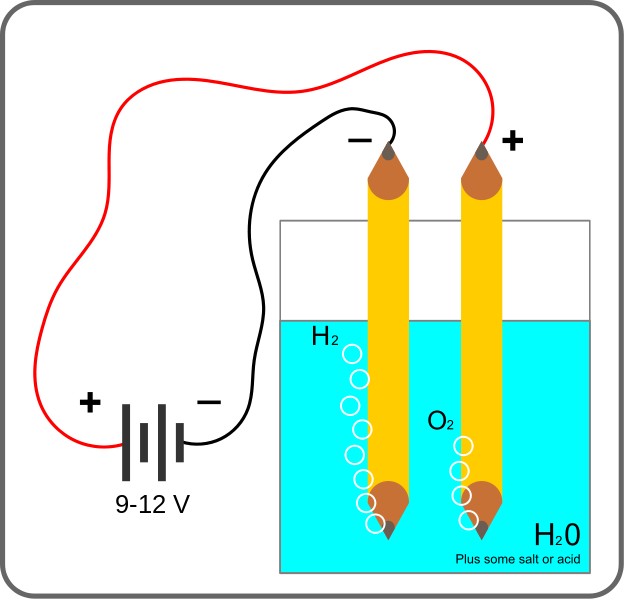
\includegraphics[width=0.5\textwidth]{photos/electrolysis.png}\\
\begin{caption}foto by Nevit Dilmen\end{caption}
\end{center}
\end{minipage} \nopagebreak
\textbf{Metode:}\\
Stel die apparaat op soos hierbo getoon. Neem waar wat gebeur.\\
\textbf{Resultaate:}\\
Jy behoort waar te neem dat borreltjies aan die punte van die potlode gevorm word. Suurstofgas word by die positiewe kant en waterstofgas word by die negatiewe kant gevorm.
\end{g_experiment}
\vspace{-.5cm}
    \section{Opsomming}
            \nopagebreak
            \label{m38120*cid7} $ \hspace{-5pt}\begin{array}{cccccccccccc}   \end{array} $ \hspace{2 pt}\raisebox{-0.2em}{
\includegraphics[height=1em]{../icons/www.pdf}} {(section shortcode: P10055 )} \par 
      \label{m38120*id311034}\begin{itemize}[noitemsep]
            \label{m38120*uid67}\item Die kleinste eenheid van materie is die \textbf{atoom}. Atome kan verbind om \textbf{verbindings} te vorm.
\label{m38120*uid68}\item 'n \textbf{Verbinding} is' n groep van twee of meer atome wat aan mekaar verbind word deur chemiese verbindings. 
\label{m38120*uid69}\item \textbf{Kovalente molekul\^{e}re struktuur} bestaan uit die wisselwerking van afsonderlike molekules.
\item \textbf{Netwerkstrukture} bestaan as 'n reuse herhalende roosterstrukture. Netwerkstrukture kan bestaan uit kovalente-, ioniese- of metaal verbindings.  
\label{m38120*uid71}\item 'n \textbf{Chemiese formule} is' n verkorte manier om 'n molekuul te beskryf deur van die simbole van die elemente in die verbinding gebruik te maak.
\label{m38120*uid72}\item Die \textbf{molekul\^{e}re formule} van 'n molekuul dui die presiese aantal atome van elke element wat in die molekuul voorkom aan.
\label{m38120*uid73}\item Die \textbf{empiriese formule} van 'n verbinding gee die relatiewe getal atome van elke element in die verbinding.
\label{m38120*uid70}\item Die struktuur van 'n verbinding kan voorgestel word deur stok-, bal-en-stok of ruimtelike modelle.
\item 'n \textbf{Stokmodel} gebruik gekleurde stokkies om verbindings voor te stel.
\label{m38120*uid75}\item 'n \textbf{Bal-en-stok-diagram} is 'n 3-dimensionele molekulêre model wat gebruik maak van "balle" om atome voor te stel en “stokkies” om die bande tussen die atome voor te stel.
\label{m38120*uid76}\item 'n \textbf{Ruimtelike} model is ook' n 3-dimensionele molekulêre model. Die atome word deur sfere voorgestel.
\label{m38120*uid77}\item In 'n molekule word atome bymekaar gehou deur \textbf{chemiese bindings}. Kovalente bindings, ioniese binding en 'n metaalbinding is voorbeelde van chemiese bindings.
\label{m38120*uid78}\item 'n \textbf{Kovalente binding} kom voor tussen nie-metaal-atome. 'n \textbf{Ioniese binding} kom voor tussen metaal en nie-metaal-atome en 'n \textbf{metaalbinding} bestaan uit die metaalatome.
\end{itemize}
\label{m38120*secfhsst!!!underscore!!!id497}
            \begin{eocexercises}{Composisie van matter}
            \nopagebreak
            \label{m38120*id311490}\begin{enumerate}[noitemsep, label=\textbf{\arabic*}. ] 
            \label{m38120*uid87}\item Gee een woord of term vir elk van die volgende beskrywings.
\label{m38120*id34411506}\begin{enumerate}[noitemsep, label=\textbf{\alph*}. ] 
            \label{m38120*uid90}\item 'n Verbinding van twee of meer atome wat as 'n eenheid optree.
\label{m38120*uid9221}\item Chemiese formule wat die relatiewe aantal atome van elke element wat in 'n molekule voorkom, gee.
\end{enumerate}
\label{m38120*uid227}\item Gee 'n definisie vir elk van die volgende terme: 
\label{m38120*id311506}\begin{enumerate}[noitemsep, label=\textbf{\alph*}. ] 
            \label{m38120*uid930}\item molekuul
\label{m38120*uid91}\item ioniese verbinding
\item kovalente netwerkstruktuur
\item empiriese formule
\item bal-en-stok-model\end{enumerate}
\label{m38120*uid92}\item Ammoniak, 'n bestanddeel in huishoudelike skoonmaakmiddels, word gemaak van een deel stikstof ($\text{N}$) en drie dele waterstof ($\text{H}$). Beantwoord die volgende vrae:
\label{m38120*id311590}\begin{enumerate}[noitemsep, label=\textbf{\alph*}. ] 
            \label{m38120*uid94}\item Is ammoniak 'n kovalente-, ioniese of metaalagtige stof?
\label{m38120*uid95}\item Skryf die molekul\^{e}re formule vir ammoniak.
\label{m38120*uid96}\item Teken 'n bal-en-stok diagram.
\label{m38120*uid97}\item Teken 'n ruimtelike diagram.
\end{enumerate}
            \label{m38120*uid11}\item In elk van die volgende, sê of die chemiese stof bestaan uit kovalente molekul\^{e}re strukture, kovalente netwerkstrukture, ioniese netwerkstrukture of metaalagtige strukture:
\label{m38120*id308055}\begin{enumerate}[noitemsep, label=\textbf{\alph*}. ] 
            \label{m38120*uid12}\item ammoniak (${\text{NH}}_{3}$)
\label{m38120*uid13}\item sinkmetaal ($\text{Zn}$)
\label{m38120*uid14}\item grafiet ($\text{C}$)
\label{m38120*uid15}\item salpetersuur (${\text{HNO}}_{3}$)
\label{m38120*uid16}\item kaliumbromied ($\text{KBr}$)
\end{enumerate}
\label{m38120*uid17}\item Verwys na die onderstaande diagram en beantwoord dan die vrae wat volg:
    \setcounter{subfigure}{0}
	\begin{figure}[H] % horizontal\label{m38120*id308155}
\begin{center}
\scalebox{0.8}{
\begin{pspicture}(-2.6,-2.4)(6,2)
\SpecialCoor
%\psgrid[gridcolor=lightgray]

\psset{unit=0.5}

\pscircle[fillcolor=red,fillstyle=solid](2,0){1.5}
\pscircle[fillcolor=blue,fillstyle=solid](0,0){2}
\pscircle[fillcolor=red,fillstyle=solid](-2,0){1.5}
% \rput(-2,0){\pscurve(1.5;45)(-1.5;180)(1.5;-45)}

\psset{unit=1.5}
\rput(4,0){\pnode(-1,0){RO}\pnode(0,0){C}\pnode(1,0){LO}
\pnode(-1,0.075){ROO}\pnode(0,0.075){CO}\pnode(1,0.075){LOO}
\psline(RO)(C)
\psline(LO)(C)
\psline(ROO)(CO)
\psline(LOO)(CO)
\rput*(C){C}
\rput*(LO){O}
\rput*(RO){O}}
\end{pspicture}
}
\end{center}
 \end{figure}       \label{m38120*id308161}\begin{enumerate}[noitemsep, label=\textbf{\alph*}. ] 
            \label{m38120*uid18}\item Identifiseer die molekule.
\label{m38120*uid19}\item Skryf die molekul\^{e}re formule vir die molekule.
\label{m38120*uid20}\item Is die molekule 'n kovalente-, ioniese of metaalagtige stof? Verduidelik.
\end{enumerate}
\label{m38120*uid21}\item Stel elk van die volgende molekules met die chemiese formule, struktuurformule en die bal-en-stok-model voor.
\label{m38120*id308228}\begin{enumerate}[noitemsep, label=\textbf{\alph*}. ] 
            \label{m38120*uid22}\item waterstof 
\item ammoniak
\item swaweldioksied
            \item stikstof
\item koolstofdioksied 
\item metaan
\item argon \end{enumerate}
\end{enumerate}
  \label{m38120**end}
\par \raisebox{-0.2em}{
\includegraphics[height=1em]{../icons/www.pdf}} Vind die antwoorde met die korkode:
 \par \begin{tabular}[h]{cccccc}
 (1.) l2e  &  (2.) l2M  &  (3.) liV  &  (4.) l2L  &   (1.) li5  &  (2.) liN  &  (3.) liR  \end{tabular}
\end{eocexercises}
